\section{Problem Definition}

% We consider the task of \textit{personalized pre-retrieval}, where the system must expand the user query before retrieval, which can not only retrieve semantically relevant user content, but also align with the user's corpus as inferred from prior interaction history. This problem is situated in settings where queries are inherently underspecified, and retrieval corpora are heterogeneous for each user.
We study \textit{personalized query expansion}, which expands underspecified queries to align with both user expression style and corpus heterogeneity informed by past interactions.

Formally, let $q$ represent the user query, and let $H = \{h_1, h_2, \dots, h_n\}$ denote the user's historical utterances, referred to as the user corpus, where each $h_i$ is a textual segment from prior conversations or interactions. The query is encoded as $\mathbf{q} = \phi(q) \in \mathbb{R}^d$, while the historical utterances are encoded into a set of corpus vectors $\mathcal{C} = \{\mathbf{c}_1, \dots, \mathbf{c}_n\}$ using a fixed encoder $\phi(\cdot)$:
\begin{equation}
\mathbf{c}_i = \phi(h_i) \in \mathbb{R}^d, \quad \forall i = 1, \dots, n.
\label{eq:c_i}
\end{equation}
% \pengyue{here, use q, but use c in equation 1. In addition, first introduce H and then introduce $\mathbf{q}= \phi(h_i) \in \mathbb{R}^d$ would be more fluent in logic} 
% Formally, let $q$ be the user query and $\mathbf{q}= \phi(q) \in \mathbb{R}^d$ be the embedding of a user-issued query, and let $H = \{h_1, h_2, \dots, h_n\}$ denote the user's historical utterances, \textit{i.e., user corpus}, where each $h_i$ is a textual segment from prior conversations or interactions. These histories are encoded into a set of courpus vectors $\mathcal{C} = \{\mathbf{c}_1, \dots, \mathbf{c}_n\} \subset \mathbb{R}^d$ via a fixed encoder $\phi(\cdot)$:

% \xdr{Formally, let $q$ represent the user query, and let $H = \{h_1, h_2, \dots, h_n\}$ denote the user's historical utterances, referred to as the user corpus, where each $h_i$ is a textual segment from prior conversations or interactions. The query is encoded as $\mathbf{q} = \phi(q) \in \mathbb{R}^d$, while the historical utterances are encoded into a set of corpus vectors $\mathcal{C} = \{\mathbf{c}_1, \dots, \mathbf{c}_n\}$ using a fixed encoder $\phi(\cdot)$:}
% \begin{equation}
% \mathbf{c}_i = \phi(h_i) \xdr{\in \mathbb{R}^d}, \quad \forall i = 1, \dots, n.
% \label{eq:c_i}
% \end{equation}

% The goal is to construct a personalized query representation $\mathbf{q}^* \in \mathbb{R}^d$ such that the retrieved set
% \begin{equation}
% \mathcal{R}(\mathbf{q}^*) = \arg\max_{\mathbf{c}_k \in \mathcal{C}} \text{sim}(\mathbf{q}^*, \mathbf{c}_k),
% \end{equation}
% reflects not only lexical-semantic relevance but also user-specific latent intent, where $\text{sim}(\cdot)$ denotes a similarity function (e.g., cosine similarity).

% The core challenge lies in the construction of $\mathbf{q}^*$ from the observable query $\mathbf{q}$ and the latent context $\mathcal{C}$. Specifically, we aim to formulate a query transformation function $f_\Theta(\mathbf{q}, \mathcal{C})$ such that:
% \begin{equation}
% \mathbf{q}^* = f_\Theta(\mathbf{q}, \mathcal{C}) = \mathbf{q} + \Delta_\text{user}(\mathbf{q}, \mathcal{C}),
% \end{equation}
% where $\Delta_\text{user}(\mathbf{q}, \mathcal{C})$ encodes a personalized adjustment that captures individual style, intent, and structural context.

The goal is to construct a personalized query representation \(\mathbf{q}^* \in \mathbb{R}^d\) that retrieves content from the user corpus \(\mathcal{C}\) not only based on lexical-semantic similarity, but also aligned with user-specific latent intent. Formally, the retrieved set is defined as:
\begin{equation}
\mathcal{R}(\mathbf{q}^*) = \text{Top}_k\left( \left\{ \text{sim}(\mathbf{q}^*, \mathbf{c}_k) \mid \mathbf{c}_k \in \mathcal{C} \right\} \right),
\end{equation}
where \(\text{sim}(\cdot)\) denotes a similarity function (e.g., cosine similarity), and \(\text{Top}_k(\cdot)\) returns the top-\(k\) most relevant items.

The core challenge lies in constructing \(\mathbf{q}^*\) from the observable query \(\mathbf{q}\) and the latent user-specific context \(\mathcal{C}\). We formulate a transformation function \(f_\Theta(\mathbf{q}, \mathcal{C})\) such that:
\begin{equation}
\mathbf{q}^* = f_\Theta(\mathbf{q}, \mathcal{C}) = \mathbf{q} + \Delta_{\text{user}}(\mathbf{q}, \mathcal{C}),
\end{equation}
where \(\Delta_{\text{user}}(\mathbf{q}, \mathcal{C})\) encodes personalized adjustments reflecting individual expression style, intent formulation, and structural semantics in the user corpus.



\begin{figure*}[th]
    \centering
    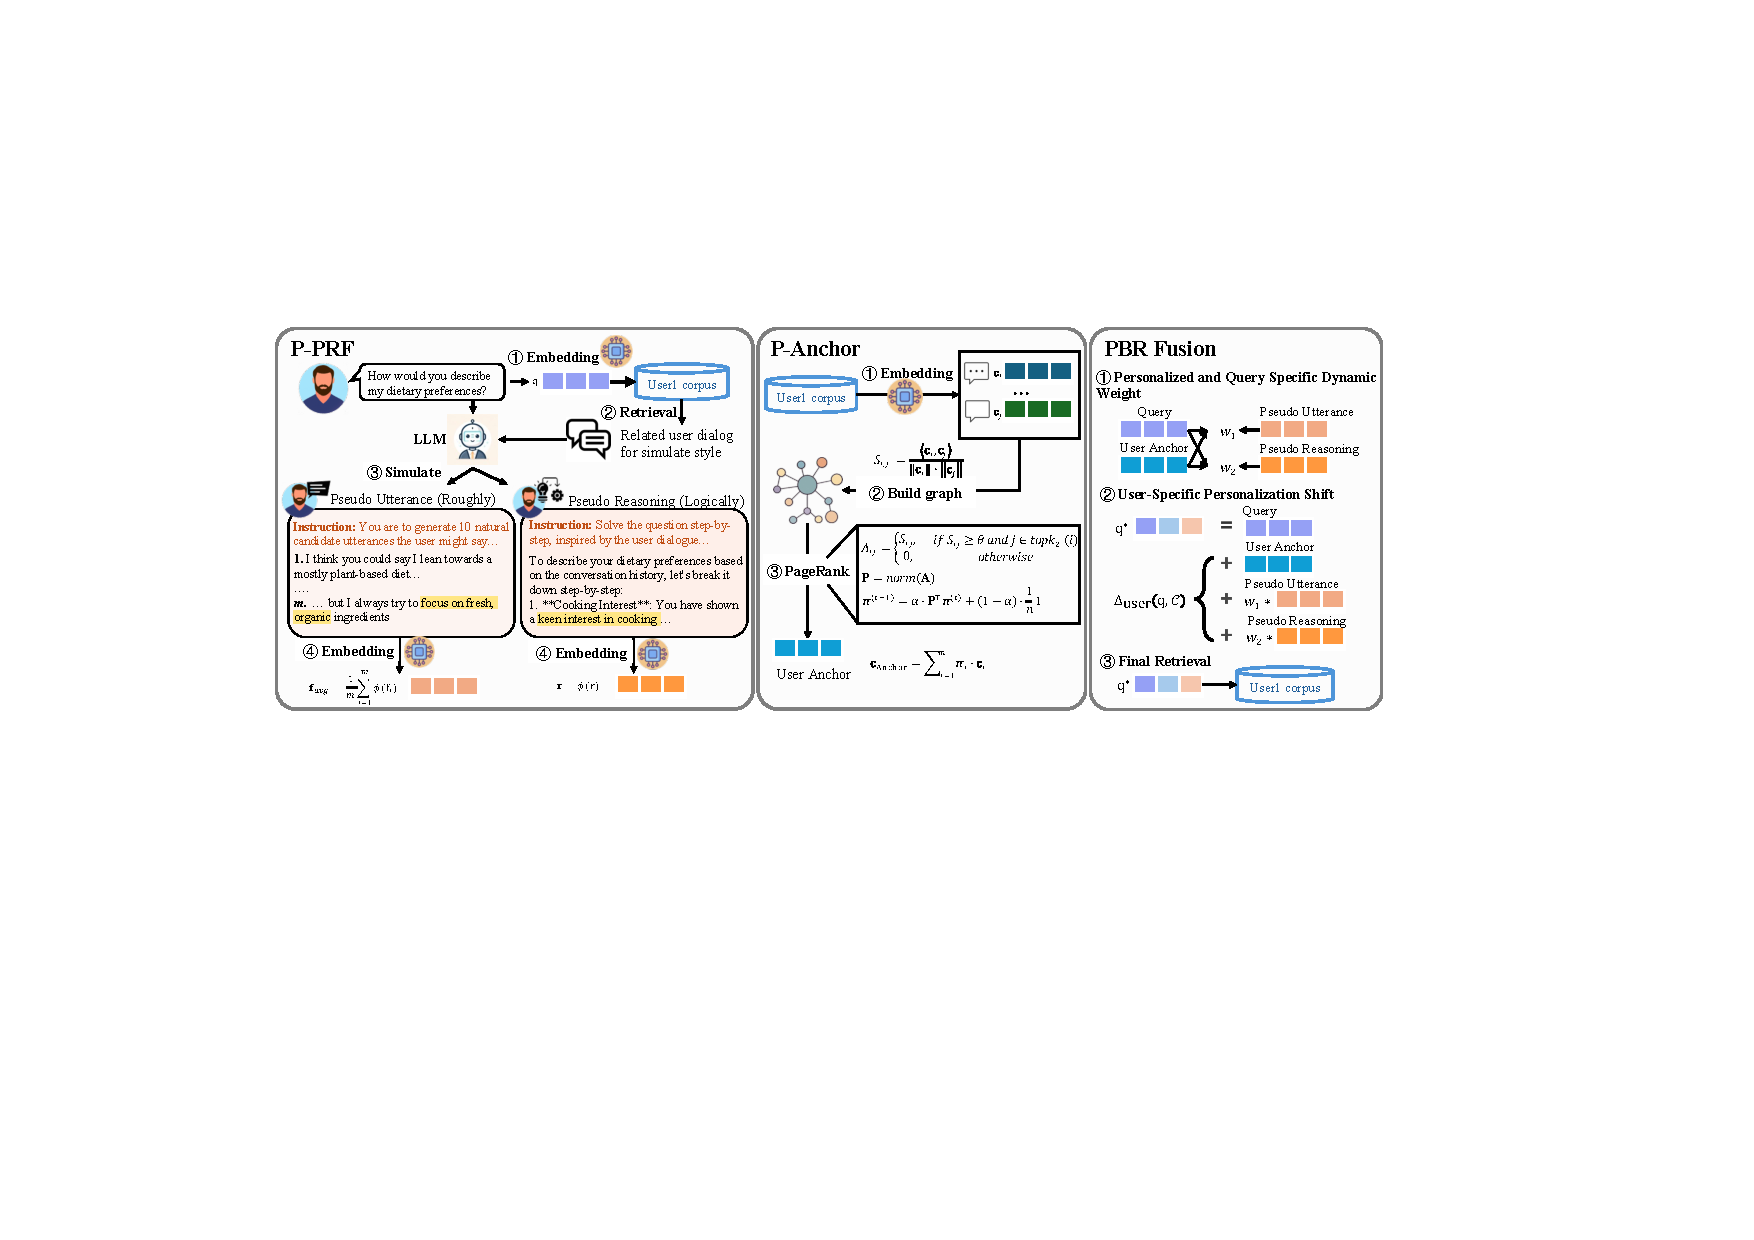
\includegraphics[width=1.00\linewidth]{figure/main_framework_final.pdf}
    \caption{Overview of PBR, which consists of three components: \textbf{P-PRF} for stylistic expansion, \textbf{P-Anchor} for structural grounding, and \textbf{PBR Fusion} module for generating the final query representation. 
    % \pengyue{add some descriptions here, for example, PBR is consisted of three modules ...}
    }
    \vspace{-10pt}
    \label{fig:main_framework}
\end{figure*}


\section{PBR Framework}



\subsection{Framework Overview}
\label{sec:framework}

As illustrated in Figure~\ref{fig:main_framework}, the \textbf{PBR} framework enhances personalized retrieval by explicitly incorporating user-specific signals into query representation before retrieval. It consists of three core modules: \textbf{P-PRF} simulates two complementary forms of feedback to generate pseudo utterances and pseudo reasoning that reflect the user's stylistic tendencies and underlying reasoning logic. \textbf{P-Anchor} constructs a semantic graph over the user's corpus and applies PageRank to identify representative anchor points that capture the corpus-level user anchor. These two sources of personalized signals are integrated via \textbf{PBR Fusion}, which computes a personalized and query-specific dynamic weight to balance the contributions of pseudo utterances and pseudo reasoning. The resulting fused representation $q^*$ reflects both user hidden style and contextual grounding, enabling accurate retrieval from the semantic index constructed over the user corpus $C$.

\subsection{P-PRF}

Generic query expansion methods often overlook the nuanced expression styles~\cite{neelakanteswara2024rags} and implicit reasoning patterns behind user expression~\cite{li2025survey}, leading to mismatches in personalized retrieval. This challenge is exacerbated when queries are ambiguous or under-specified, requiring systems to infer intent beyond surface forms. Existing solutions typically apply uniform expansion strategies, failing to adapt to user-specific language signals.

To address these limitations, \textbf{P-PRF} simulates user-specific signals before retrieval by simulating personalized feedback in two complementary forms: \emph{roughly} via stylistic utterances, and \emph{logically} via intent reasoning. Rather than using the full user history $H$, we retrieve a task-relevant subset $H_q$  based on semantic similarity:
\begin{equation}
H_q= \text{TopK}\big(\{\text{sim}(\mathbf{q}, \mathbf{c}_t)\}_{t=1}^n\big), \quad |H_q| = k_1,
\end{equation}
where $\mathbf{q}$ and $\mathbf{c}_t$ are the embeddings of the query and past utterances. This subset captures salient contextual-aware user traits for downstream simulation.

\paragraph{Pseudo Utterance Generation (Roughly)}  
To simulate user-specific expression patterns, we employ a large language model $\mathcal{G}^{\text{utt}}_{\text{LLM}}$ to generate $m$ pseudo utterances conditioned on the original query $q$ and user dialogue history $H_q$. Each utterance $f_i$ is designed to reflect how the user might naturally articulate the query, capturing stylistic nuances such as tone, verbosity, and phrasing:
\begin{equation}
F = \{f_1, \dots, f_m\} = \mathcal{G}^{\text{utt}}_{\text{LLM}}(q, H_q), \quad \mathbf{f}_{\text{avg}} = \frac{1}{m} \sum_{i=1}^{m} \phi(f_i),
\end{equation}
where $\phi(f_i)$ denotes the embedding of the $i$-th utterance and $\mathbf{f}_{\text{avg}}$ is their mean representation.
% \yc{what about $m$, and how to construct the $\mathcal{G}^{\text{utt}}_{\text{LLM}}$}

\paragraph{Pseudo Reasoning Generation (Logically)}  
Beyond surface expression, effective personalization also requires modeling the user’s implicit reasoning process. We define $\mathcal{G}^{\text{rea}}_{\text{LLM}}$ as a parallel simulating pipeline to elicit a step-by-step rationale $r$ of user expression:
\begin{equation}
r = \mathcal{G}^{\text{rea}}_{\text{LLM}}(q, H_q), \quad \mathbf{r} = \phi(r).
\end{equation}
This rationale introduces logical cues that are often absent from surface queries, thereby providing a complementary semantic signal to guide expansion alignment.


\begin{table*}[t]
\centering
% \pengyue{can this table move to the next page? and the suboptimal results should be underlined.}
\small
\setlength\tabcolsep{2.75pt}  %可以控制列间距
\renewcommand{\arraystretch}{0.80} %可以控制行间距
% \resizebox{175mm}{!}{
\begin{tabular}{lcccccccccccccc}
\toprule
 \textbf{Method} & \multicolumn{2}{c}{\textbf{Base}} & \multicolumn{2}{c}{\textbf{HyDE}} & \multicolumn{2}{c}{\textbf{Query2Term}} & \multicolumn{2}{c}{\textbf{MILL}} & \multicolumn{2}{c}{\textbf{CoT}} & \multicolumn{2}{c}{\textbf{ThinkQE}} & \multicolumn{2}{c}{\textbf{PBR (Ours)}} \\
\cmidrule(r){2-3} \cmidrule(r){4-5} \cmidrule(r){6-7} \cmidrule(r){8-9} \cmidrule(r){10-11} \cmidrule(r){12-13} \cmidrule(r){14-15}
Metrics & R@5 & N@5 & R@5 & N@5 & R@5 & N@5 & R@5 & N@5 & R@5 & N@5 & R@5 & N@5 & R@5 & N@5 \\
\midrule
\rowcolor{gray!15}
\multicolumn{15}{c}{\textit{multi-qa-MiniLM-L6-cos-v1}} \\
\textbf{Overall} & 0.4484 & 0.3669 & 0.3464 & 0.2945 & 0.3584 & 0.3060 & 0.3200 & 0.3254 & 0.3627 & 0.3000 &\underline{0.4791}&\underline{0.3902}& \textbf{0.5035} & \textbf{0.4201} \\
Basic information & 0.4515 & 0.3088 & 0.3106 & 0.2395 & 0.3424 & 0.2614 & 0.2879 & 0.2337 & 0.3424 & 0.2454 &\underline{0.4606}&\underline{0.3265}& \textbf{0.5091} & \textbf{0.3647} \\
Preference (hard) & 0.3659 & 0.3759 & 0.3122 & 0.3079 & 0.3659 & 0.3491 & 0.2927 & \underline{0.4250} & 0.3171 & 0.3335 &\textbf{0.4195}&\textbf{0.4310}& \underline{0.4049} & 0.4175 \\
Social & 0.4852 & 0.4356 & 0.3909 & 0.3259 & 0.3494 & 0.3144 & 0.3808 & 0.3923 & 0.4009 & 0.3320 &\underline{0.5503}&\underline{0.4554}& \textbf{0.5541} & \textbf{0.4914} \\
Preference (easy) & 0.4904 & 0.4582 & 0.4615 & 0.4422 & 0.4327 & 0.4095 & 0.3750 & 0.4195 & 0.4423 & 0.4133 &\underline{0.5064}&\underline{0.4626}& \textbf{0.5321} & \textbf{0.5129} \\
\midrule
\rowcolor{gray!15}
\multicolumn{15}{c}{\textit{all-MiniLM-L6-v2}} \\
\textbf{Overall} & 0.3783 & 0.3074 & 0.3747 & 0.3144 & 0.3908 & 0.3256 & 0.3030 & 0.3059 & 0.3721 & 0.3098 &\underline{0.3861}&\underline{0.339}3& \textbf{0.4516} & \textbf{0.3855} \\
Basic information & 0.3515 & 0.2644 & \underline{0.4015} & \underline{0.2975} & 0.3894 & 0.2914 & 0.3030 & 0.2547 & 0.3455 & 0.2696 &0.3455&0.2677& \textbf{0.4515} & \textbf{0.3485} \\
Preference (hard) & \underline{0.4000} & 0.3547 & 0.3512 & 0.3561 & 0.3805 & 0.3798 & 0.3220 & \underline{0.4171} & 0.3463 & 0.3490 &0.3366&0.3486& \textbf{0.4341} & \textbf{0.4352} \\
Social & 0.3921 & 0.3048 & 0.2805 & 0.2435 & 0.3984 & 0.3163 & 0.2638 & 0.2829 & 0.4160 & 0.3046 &\textbf{0.4780}&\textbf{0.4334}& \underline{0.4494} & \underline{0.3777} \\
Preference (easy) & 0.4295 & 0.4199 & \textbf{0.4904} & \underline{0.4646} & 0.3974 & 0.4038 & 0.3526 & 0.3944 & 0.4359 & 0.4285 &0.4487&0.4357& \underline{0.4840} & \textbf{0.4800} \\
\midrule
\rowcolor{gray!15}
\multicolumn{15}{c}{\textit{bge-base-en-v1.5}} \\
\textbf{Overall} & \underline{0.3738} & 0.3015 & 0.3108 & 0.2597 & 0.3007 & 0.2497 & 0.2791 & 0.2869 & 0.3199 & 0.2642 &0.3643&\underline{0.3156}& \textbf{0.4029} & \textbf{0.3402} \\
Basic information & \underline{0.3970} & 0.2748 & 0.2955 & 0.2051 & 0.3000 & 0.1955 & \underline{0.2879} & 0.2319 & 0.3152 & 0.2052 &0.3152&0.2430& \textbf{0.4121} & \textbf{0.3057} \\
Preference (hard) & 0.3268 & 0.3343 & 0.3073 & 0.3148 & 0.2976 & 0.3186 & 0.2244 & 0.3566 & 0.3073 & 0.3281 &\underline{0.3463}&\underline{0.3635}& \textbf{0.3707} & \textbf{0.3889} \\
Social & 0.3204 & 0.2799 & 0.2714 & 0.2443 & 0.2852 & 0.2503 & 0.2752 & 0.3004 & 0.2965 & 0.2647 &\textbf{0.4261}&\textbf{0.3735}& \underline{0.3657} & \underline{0.3089} \\
Preference (easy) & 0.4583 & 0.4065 & 0.4615 & \underline{0.4356} & 0.3397 & 0.3693 & 0.3365 & 0.3819 & 0.4071 & 0.4117 &\underline{0.4744}&0.4289& \textbf{0.4904} & \textbf{0.4734} \\
\midrule
\textbf{Overall Average} & 0.4002 & 0.3253 & 0.3440 & 0.2895 & 0.3500 & 0.2938 & 0.3007 & 0.3061 & 0.3295 & 0.3121 &\underline{0.4098}& \underline{0.3484}& $\textbf{0.4527}^*$ & $\textbf{0.3819}^*$\\
\bottomrule
\end{tabular}
% }
\caption{Retrieval performance in \textbf{PersonaBench}. The best results are in \textbf{bold}, and the second-best results are \underline{underlined}. ``\textbf{{\Large *}}'' indicates the statistically significant improvements (i.e., two-sided t-test with $p<0.05$) over the best baseline. }
\label{tab:main_results}
\vspace{-10pt}
\end{table*}

\subsection{P-Anchor}
% While P-PRF simulates personalized signals in expression and reasoning, 
% Existing method are often expand query to retrieval in the unified RAG data corpus, it lacks explicit grounding in the structural distribution of the user’s corpus. 
Existing methods are often designed to retrieve from a unified RAG corpus, lacking explicit grounding in the structural organization of individual user corpora~\cite{tan2025personabench,wu2025longmemeval}.
% \zc
To address this, we propose \textbf{P-Anchor}, a structure-aware module that captures corpus-level preferences by identifying semantically central regions within a graph-structured user space.

\paragraph{Graph Construction from User Corpus.}
We represent the user's prior corpus—such as interaction records with AI assistants—as a semantic graph $G = (\mathcal{C}, \mathcal{E})$, following previous study~\cite{tang2025llm4tag}, where $\mathcal{C}$  and $\mathcal{E}$ denote the sets of nodes and edges, respectively. 
% \yc{$\mathcal{C}$ has been mentioned in many places, are they the same concept?} 
The set of nodes $\mathcal{C}$ consists of history corpus vectors, where each node $\mathbf{c}_i$ as in Eq. \eqref{eq:c_i} represents an encoded segment. The edges $\mathcal{E}$ are established based on pairwise similarity between the nodes.
For each pair, we compute cosine similarity:
\begin{equation}
S_{ij} = \frac{\langle \mathbf{c}_i, \mathbf{c}_j \rangle}{\|\mathbf{c}_i\| \cdot \|\mathbf{c}_j\|}.
\end{equation}
We construct a sparse adjacency matrix $A$ to represent the structural links within the user corpus, which retains only the top-$k_2$ neighbors exceeding a similarity threshold $\theta$:
% A sparse adjacency matrix $A$ retains only the top-$k_2$ neighbors exceeding a threshold $\theta$, preserving salient structural links:
% \pengyue{k has been used before} 
\begin{equation}
A_{ij} = 
\begin{cases}
S_{ij}, & \text{if } S_{ij} \geq \theta \text{ and } j \in \text{top-}k_2(i), \\
0, & \text{otherwise}.
\end{cases}
\end{equation}

\paragraph{Graph-Based Anchor Representation.}
% \pengyue{give a citation, or change to ``following PageRank''}
We following PageRank~\cite{page1999pagerank,haveliwala2002topic}  over $G$ to estimate a stationary distribution $\boldsymbol{\pi}$ reflecting node centrality. Let $\mathbf{P}=norm(\mathbf{A})$ be the row-normalized transition matrix, then:
% \begin{equation}
% P_{ij} = \frac{A_{ij}}{\sum_{j'} A_{ij'} + \epsilon}.
% \end{equation}
\begin{equation}
\boldsymbol{\pi}^{(t+1)} = \alpha \cdot \mathbf{P}^\top \boldsymbol{\pi}^{(t)} + (1 - \alpha) \cdot \frac{1}{n} \mathbf{1}.
\end{equation}
The user anchor is computed as a weighted aggregation:
\begin{equation}
\mathbf{c}_{\text{Anchor}} = \sum_{i=1}^{n} \boldsymbol{\pi}_i \cdot \mathbf{c}_i.
\end{equation}
% \xdr{$\mathbf{c}_{\text{Anchor}}$ may be better} 
This representation encodes structurally central semantics from the user's corpus, anchoring the query in a context-aware and personalized semantic space.




\subsection{PBR Fusion}  

To synthesize the signals captured in P-PRF and P-Anchor, we design a fusion mechanism that integrates stylistic pseudo-feedback with the query and user anchor. Recognizing that the utility of pseudo-feedback varies across users and queries—depending on individual expression patterns and the semantic openness of the query—we introduce a \textit{personalized and query-specific dynamic weight} that balances the contribution of P-PRF according to its semantic proximity to both the original query $\mathbf{q}$ and the corpus anchor $\mathbf{c}_{\text{Anchor}}$. Specifically, we compute two weights $w_1$ and $w_2$ to quantify the semantic alignment of the pseudo-utterance and reasoning feedback, respectively:
% \yc{uninformative descriptions, should elaborate the rationale behind this fusion design, especially the relationship between c anchor and w1 or w2}
\begin{equation}
w_1 = 1 + \text{sim}\left( \frac{\mathbf{q} + \mathbf{c}_{\text{Anchor}}}{2}, \mathbf{f}_{\text{avg}} \right), \quad
\end{equation}
\begin{equation}
w_2 = 1 + \text{sim}\left( \frac{\mathbf{q} + \mathbf{c}_{\text{Anchor}}}{2}, \mathbf{r} \right),
\end{equation}
% \pengyue{the end sign should be a comma or a period? Please confirm this point, then check the whole paper.} \yy{[I think depend on the expression, if the equation is the final of the sentence, it should be period, otherwise the comma]}
where $\text{sim}(\cdot)$ denotes cosine similarity. The additive constant ensures positivity and smooth interpolation.

Then, we define a user-specific personalization shift as:
\begin{equation}
\Delta_\text{user}(\mathbf{q}, \mathcal{C}) = \mathbf{c}_{\text{Anchor}} + w_1 \cdot \mathbf{f}_{\text{avg}} + w_2 \cdot \mathbf{r},
\end{equation}
and construct the final personalized query embedding as:
\begin{equation}
\mathbf{q}^* = \mathbf{q} + \Delta_\text{user}(\mathbf{q}, \mathcal{C}).
\end{equation}

The resulting query $\mathbf{q}^*$ incorporates user-specific semantics from both style and structure. It encodes not only the immediate surface form of the input query, but also latent stylistic preferences, goal-driven reasoning, and historically salient corpus signals.


\paragraph{Final Retrieval.}  
We retrieve from the user corpus $\mathcal{C}$ using \texttt{faiss}-based~\cite{douze2024faiss} nearest neighbor search with the fused query vector $\mathbf{q}^*$. This process leverages embedding-level alignment to recover user-relevant content.
% \pengyue{citation} 
